\documentclass{article}
\usepackage{listings}
\usepackage{graphicx}
\usepackage[slovene]{babel}
\usepackage{color}
\usepackage{amsmath}
\usepackage[usenames,dvipsnames]{xcolor}
\usepackage[hidelinks]{hyperref}
\usepackage{subcaption}
\usepackage{float}
\usepackage{rotating} 
\usepackage{hyperref}
\usepackage{caption}
\usepackage{siunitx}
\graphicspath{{./images/}}

\setlength{\parindent}{0pt}

\begin{document}

\title{Matematično-fizikalni praktikum \\[3mm] \large Naloga 9}
\author{Luka Papež}
\date{1.\ januar 2025}

\begin{center}
    
\includegraphics[width=8cm]{logo-fmf.png}
\end{center}

{
    \let\newpage\relax
    \maketitle
}

\maketitle
\newpage
\section{Naloga}
\begin{itemize}
  \item Reši difuzijsko enačbo v eni razsežnosti $x\in [0,a]$
z začetnim pogojem po plasti gaussovsko porazdeljene temperature
\begin{equation*}
  T(x,0) \propto \mathrm{e}^{-(x-a/2)^2 / \sigma^2}
\end{equation*}
(izberi razumne vrednosti za $D$, $a$ in $\sigma$)
in
\begin{enumerate}
 \item periodičnim robnim pogojem $T(0,t) = T(a,t)$.
 \item homogenim Dirichletovim robnim pogojem $T(0,t) = T(a,t)=0$.
\end{enumerate}
po Fourierovi metodi.
\item Kolokacijsko metodo uporabi ob Gaussovem začetnem pogoju
in homogenih Dirichletovih robnih pogojih $T(0,t)=T(a,t)=0$ ter primerjaj obe metodi.
\end{itemize}
\section{Uvod}
Za reševanje začetnih problemov s parcialnimi diferencialnimi
enačbami (PDE) imamo na voljo dva obsežna razreda metod.
Pri {\sl diferenčnih metodah\/} na neki način aproksimiramo
časovne in krajevne parcialne odvode s končnimi diferencami.
Reševanje PDE nato prevedemo na reševanje algebrajskih enačb
ali sistemov enačb za približne vrednosti funkcij, ki v teh
diferencah nastopajo.  Diferenčne metode spoznamo pri
naslednji vaji.  Pri tej vaji obravnavamno {\sl spektralne metode\/}:
pri njih iskano rešitev formalno izrazimo z nekim naborom funkcij,
nato pa v času spremljamo koeficiente v takem razvoju.  Kako se
selimo med krajevno in časovno sliko problema, je odvisno
od posamezne metode.  Osnovne prijeme spoznamo ob Fourierovi
metodi in  metodi končnih elementov s kubičnimi $B$-zlepki ($B$-splines).

Fizikalno ozadje naj bo enorazsežna difuzijska enačba,
ki opisuje na primer temperaturno polje $T(x,t)$ v homogeni
neskončni plasti s končno debelino $a$ brez izvorov toplote:
\begin{equation*}
\Pd{T}{t} = D\Pd[2]{T}{x}
 \>, \qquad 0\le x \le a \>, \qquad D={\lambda\over \rho c} \>.
\end{equation*}
Temperaturo v poljubni točki $x$ ob času $t$ izrazimo
s Fourierovo vrsto
\begin{equation*}
T(x,t) \simeq \sum_{k=0}^{N-1} \widetilde{T}_k(t)
e^{-2\pi\mathrm{i} f_k x} \>,
\end{equation*}
kjer je $f_k = k/a$, torej
\begin{equation*}
\sum_k {\partial\widetilde{T}_k(t)\over\partial t}\,
\mathrm{e}^{-2\pi\mathrm{i} f_k x} =
D \sum_k (-4\pi^2 f_k^2) \, \widetilde{T}_k(t) \,
\mathrm{e}^{-2\pi\mathrm{i} f_k x} \>.
\end{equation*}
Od tod sledi evolucijska enačba za Fourierove koeficiente
\begin{equation}
{\partial\widetilde{T}_k(t)\over\partial t} =
D \, (-4\pi^2 f_k^2) \, \widetilde{T}_k(t) \>.
\label{eq:num}
\end{equation}
Pogosto uporabimo spektralno reprezentacijo za krajevni odvod,
medtem ko časovni korak naredimo z neko eksplicitno integracijsko
shemo, na primer kar po Eulerju
\begin{equation}
\widetilde{T}_k(t+h) = \widetilde{T}_k(t)
+ h D (-4\pi^2 f_k^2) \widetilde{T}_k(t) \>.
\label{ffteuler}
\end{equation}
Reprezentacijo $T(x,t)$ v običajnem prostoru nato dobimo
z obratno Fourierovo transformacijo.

\bigskip

Tu lahko v splošnem časovni korak izvedeš po Eulerju, v tem konkretnem primeru
pa obstaja tudi enostavna analitična rešitev enačbe \ref{eq:num}, ki jo lahko uporabiš za primerjavo.
V numerični metodi tako najprej izračunaj Fourierovo reprezentacijo $\widetilde{T}_k(0)$
začetnega pogoja, nato pa jo po Eulerju evolviraj v času.
Pri tem moraš paziti na stabilnost Eulerjeve diferenčne sheme:
pri katerem koli koraku mora veljati
\begin{equation*}
\left\vert \,
{\widetilde{T}_k(t+h)\over \widetilde{T}_k(t)} \,\right\vert
= \left\vert\, 1 + hD(-4\pi^2 f_k^2)\, \right\vert < 1 \>.
\end{equation*}

Nekaj pozornosti zahteva tudi diskretizacija: za vsak $k$
seveda velja  $-f_\mathrm{Nyquist} < f_k < f_\mathrm{Nyquist}$ in s tem povezan
mo\v zen pojav \emph{aliasinga} (Kaj je že to?). Ta pojav lahko \v studira\v s,
\v ce se spomni\v s, da obstaja analiti\v cna re\v sitev FT Gaussove funkcije (je spet Gaussova funkcija) - kaj se z le-to dogaja znotraj dovoljenega frekvenčnega intervala?
\v Ce izbereš veliko število točk, je seveda smiselno uporabiti kar algoritem FFT.
Temperaturni profil $T_j(t)\equiv T(x,t)$ ob poljubnem času
nato dobiš z inverzno FFT.

\bigskip

Pri razvoju $T(x,t)$ nismo omejeni
na trigonometrične funkcije.  Rešitev PDE na $0\le x\le a$
lahko aproksimiramo tudi z drugačno vrsto funkcij,
na primer kubičnimi $B$-zlepki,
\begin{equation}
T(x,t) = \sum_{k=-1}^{N+1} c_k(t) B_k(x) \>,
\label{Tcolloc}
\end{equation}
kjer je $B_k(x)$ kubični zlepek s središčem okrog $x=x_k$.
aastnosti $B$-zlepkov so navedene v dodatku.  Tako zasnujemo
{\sl metodo končnih elementov}, s \emph{kolokacijskim pogojem}, da naj se zlepek
ujema z rešitvijo v določenih izbranih točkah.  Podobno kot pri Fourierovi metodi
tudi pri tej metodi zahtevamo, da razvoj~(\ref{Tcolloc})
zadošča osnovni PDE in robnim pogojem.  Razvoj~(\ref{Tcolloc})
vstavimo v PDE in izvrednotimo rezultat pri $x=x_j$.
(Interval $[0,a]$ diskretiziramo na $N$ podintervalov širine
$\Delta x$ s točkami $x_j=j{\Delta x}$, kjer je $j=0,1,\ldots,N$.
Za kolokacijo je smiselno izbrati enake točke kot za diskretno
mrežo.)  Tako dobimo
$$
\sum_{k=-1}^{N+1} \dot{c}_k(t) B_k(x_j) =
D \sum_{k=-1}^{N+1} c_k(t) B_k''(x_j) \>, \quad j = 0,1,\ldots,N \>.
$$
Upoštevamo lastnosti $B$-zlepkov in dobimo sistem
diferencialnih enačb za koeficiente $c_j(t)$:
$$
\dot{c}_{j-1}(t) + 4\dot{c}_j(t) + \dot{c}_{j+1}(t)
= {6D\over{\Delta x}^2} \left(c_{j-1}(t) - 2c_j(t) + c_{j+1}(t) \right) \>,
$$
kjer je $j=0,1,\ldots,N$.  Iz robnega pogoja pri $x=0$
ugotovimo $c_{-1} = -4c_0 - c_1$. Če dodamo še zahtevo za 'naravni' kubični
zlepek, da je na robu $\sum_{k=-1}^{N+1} c_k(t) B_k''(x=(0,a))=0$, sledi
 $c_0=c_N=0$ in $c_{-1}=-c_1$ ter $c_{N-1}=-c_{N+1}$.
Reševanje enačbe~(\ref{Tcolloc}) smo torej prevedli
na reševanje matričnega sistema
$$
{\bi A}\frac{d\vec{c}}{dt} = {\bi B}\vec{c} \>,
$$
kjer je
$$
{\bi A} = \left(
\begin{array}{ccccccc}
4 & 1 \cr
1 & 4 & 1 \cr
  & 1 & 4 & 1 \cr
  &   &   & \vdots \cr
  &   &   & 1 & 4 & 1 & \cr
  &   &   &   & 1 & 4 & 1 \cr
  &   &   &   &   & 1 & 4
\end{array}
\right) \>, \qquad
{\bi B} = {6D\over{\Delta x}^2} \left(
\begin{array}{rrrrrrr}
-2 & 1 \cr
1 & -2 & 1 \cr
  & 1 & -2 & 1 \cr
  &   &   & \vdots \cr
  &   &   & 1 & -2 & 1 & \cr
  &   &   &   & 1 & -2 & 1 \cr
  &   &   &   &   & 1 & -2
\end{array}
\right)
$$
in $\vec{c} = (c_1(t), c_2(t), \ldots c_{N-1}(t))^\mathrm{T}$.
Začetni pogoj za PDE je $T(x_j,0) = f(x_j)$, torej je začetni
približek za kolokacijsko aproksimacijo
$$
{\bi A}\vec{c}^{\>0} = \vec{f} \>,
$$
kjer je $\vec{f}=(f(x_1),f(x_2),\ldots,f(x_{N-1}))^\mathrm{T}$.
To zdaj rešujemo s kako metodo, ki jo poznamo iz prejšnjih
nalog, recimo z eksplicitno Eulerjevo metodo: ob zaporednih
časih $n{\Delta t}$ dobimo
$$
\vec{c}^{\>n+1} = \vec{c}^{\>n} + {\Delta t}{ A}^{-1}{ B}\vec{c}^{\>n}
 = ( { 1} + {\Delta t}{ A}^{-1}{ B})\vec{c}^{\>n} \>.
$$
Ob poljubnem času nato dobimo temperaturni profil tako,
da znova izračunamo vsoto.
Ker nam je že znano, da je Eulerjeva ob predolgih časovnih korakih
lahko nestabilna, lahko uporabimo stabilno implicitno metodo,
kjer v vsakem časovnem koraku rešujemo
$$
  \left( { A} - \frac{\Delta t}{2}{ B}\right)\vec{c}^{\>n+1} \>
 = \left( { A} + \frac{\Delta t}{2}{ B}\right)\vec{c}^{\>n} \>.
$$
\newpage
\section{Rešitev}
\subsection{Fourirjeva metoda}
V tej nalogi rešujemo difuzijsko enačbo s pomočjo katere bomo opisali širjenje temperature glede na gaussov začetni pogoj, ki ga za nadaljno uporabo definiramo v obliki  $T(x, 0) = e^{\frac{(x-\bar{x})^2}{\sigma^2}}$. Za reševanje parcialne diferencialne enačbe ostanejo trije parametri, ki jih za nadaljno reševanje nastavimo na $D=1$ $\sigma=0.25$ in $x_0=0.5$. Tako lahko s pomočjo fourirjeve transformacije najprej izračunamo koeficiente $c_k(t)$ ob $t=0$, nato pa jih preko analitične rešitve $c_k(t)=c_k(0)e^{-4\pi^2f_k D t}$ časovno propagiramo in s pomočjo inverzne fourirjeve transformacije dobimo rešitev ob poljubnem času. 
\begin{figure}[H]
    \centering
    \begin{subfigure}{0.45\textwidth}
        \centering
        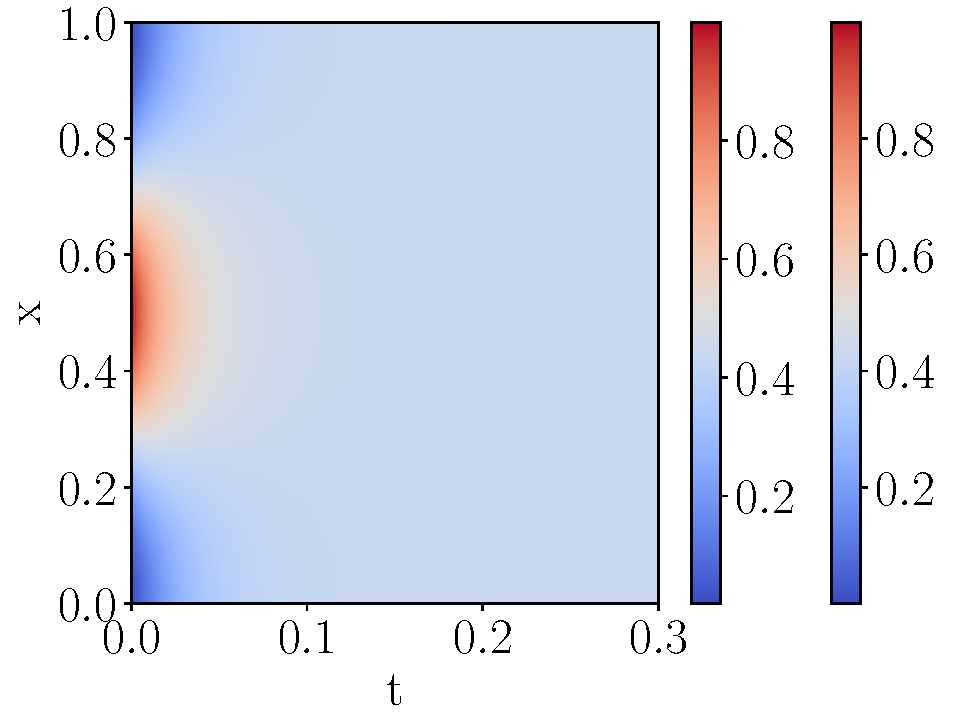
\includegraphics[width=\linewidth]{fourier2d.pdf}
    \end{subfigure}
    \hspace{0.5cm}
    \begin{subfigure}{0.45\textwidth}
        \centering
        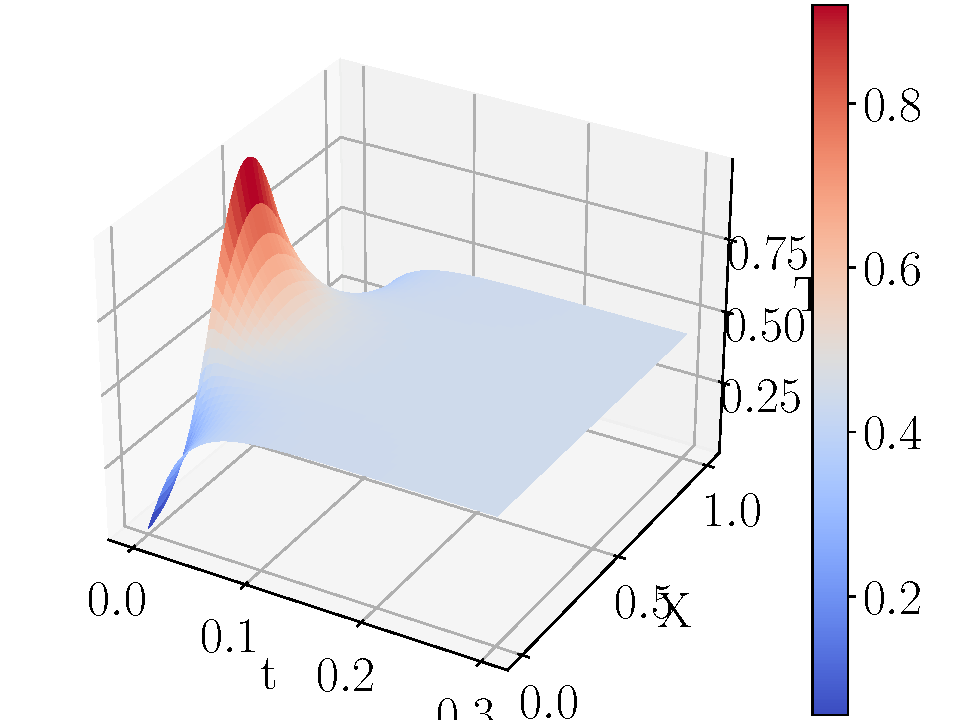
\includegraphics[width=\linewidth]{fourier3d.pdf}
    \end{subfigure}
	\caption{Rešitev difuzijske enačbe s periodičnimi pogoji s Fourirjevo metodo}
\end{figure}
Kot pričakovano temperatura postopoma konvergira h konstanti. Sta pa zgornja grafa tudi zgledna primera, kako nam različne vizualizacije podajo različne podatke. V dvo dimenzionalnem grafu so spremembe temperature čez prostor in čas precej lažje razvidne, a v njej oblika funkcije temperature v določenem trenutku ni tako očitna. Na tri dimenzionalnem grafu pa hitro opazimo, da se skozi čas približno ohranja oblika Gaussove funkcije. Ob prej opisanem postopku dobimo periodične pogoje, ki izhajajo iz lastnosti Fourirjeve transformacije, ki vedno privzame periodičnost. Da bi izpolnili Dirichletove pogoje $T(0,t)=T(a,t)=0$ pa moramo opraviti liho razširitev začetnega pogoja oziroma z drugimi besedami liho zrcaljenje funkcije čez izhodišče.
\begin{figure}[H]
    \centering
    \begin{subfigure}{0.45\textwidth}
        \centering
        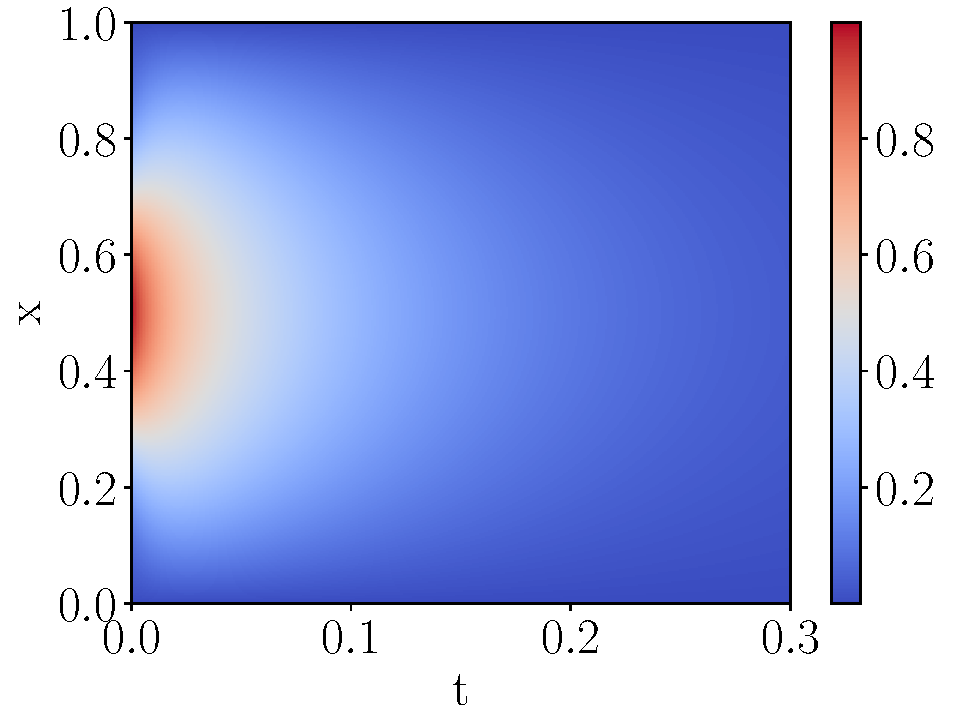
\includegraphics[width=\linewidth]{hom_fourier2d.pdf}
    \end{subfigure}
    \hspace{0.5cm}
    \begin{subfigure}{0.45\textwidth}
        \centering
        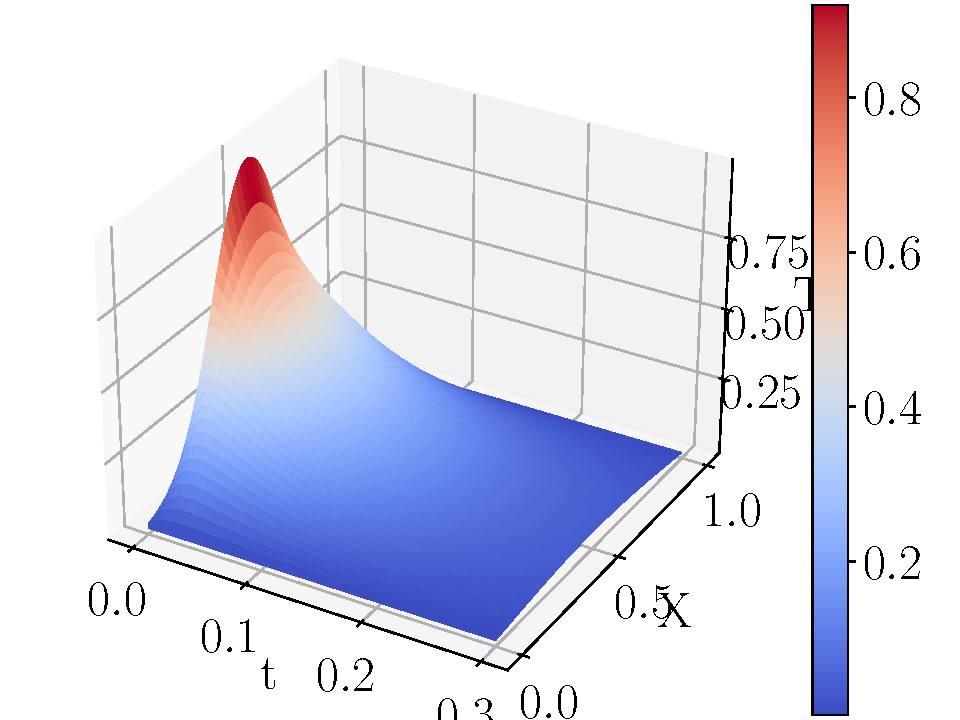
\includegraphics[width=\linewidth]{hom_fourier3d.pdf}
    \end{subfigure}
	\caption{Rešitev difuzijske enačbe z Dirichletovimi pogoji s Fourirjevo metodo}
\end{figure}

\medskip

Reševanje s Fourirjevo metodo pa na žalost ni šlo tako tekoče kot je bilo do sedaj predstavljeno. Najprej je na prvi pogled prišla dokaj pravilna rešitev, a sem po implementaciji metode, ki sledi opazil, da se rešitvi ne ujemata. Tako sem najprej odkril manjšo napako, nato pa še tisto o kateri bi rad povedal nekaj več. Vhod v hitro Fourirjevo transformacijo je v našem primeru namreč realen, kar pomeni, da so negativne frekvence le prezrcaljene pozitivne. Hitra fourirjeva transformacija, ki jo ponudi numpy pa namreč porazdeli rezultate tako, da sledijo najprej pozitivne frekvence nato pa še negativne. To smo najprej v časovni propagaciji izpustili in tako uporabili napačne konstante $k$. \\
Za odpravo napake se moramo najprej seveda spomniti na Nyquistovo frekvenco, ki je polovica frekvence vzorčenja in predstavlja maksimalno zaznavno frekvenco Fourirjeve transformacije. S tem podatkom lahko zdaj popravimo napačne frekvence, ki smo jih uporabljali pri časovni propagaciji koeficientov vsote. Iz vseh napisanih razmiselkov tako sledi, da so frekvence za prvo polovico izhoda hitre Fourirjeve transformacije $k/a$, kjer je $k=0,1...n/2-1$ in za drugo polovico ustrezajo naslednje vrednosti $k=-n/2,...,-1$. Lahko pa našo nalogo še poenostavimo in pohitrimo tako, da namesto `numpy.fft.fft` uporabimo funkcijo, ki je namenjena računanju z realnim vhodom `numpy.fft.rfft` in njej pripadajoč inverz. Tako se naše delo propagiranja poenostavi na le prej omenjeno prvo polovico frekvenc.
\subsection{Metoda končnih diferenc}
Poglejmo si še metodo končnih diferenc. Z namenom stabilnosti uporabljamo Eulerjevo implicitno metodo. Začetne vrednosti izračunamo s pomočjo inverza za katerega se lahko hitro prepričamo, da obstaja. Enako storimo tudi pri računanju Eulerjeve implicitne metode. Za reševanje teh enačb obstajajo tudi boljše metode, ki se jih bomo glede na namig iz predavanj lotili v naslednji nalogi. Rezultati so na videz po nekaj dela seveda enaki kot pri Fourirjevi metodi. Zato primerjajmo obe rešitvi podrobno in poglejmo kje se med njima pojavijo odstopanja.
\begin{figure}[H]
    \centering
    \begin{subfigure}{0.45\textwidth}
        \centering
        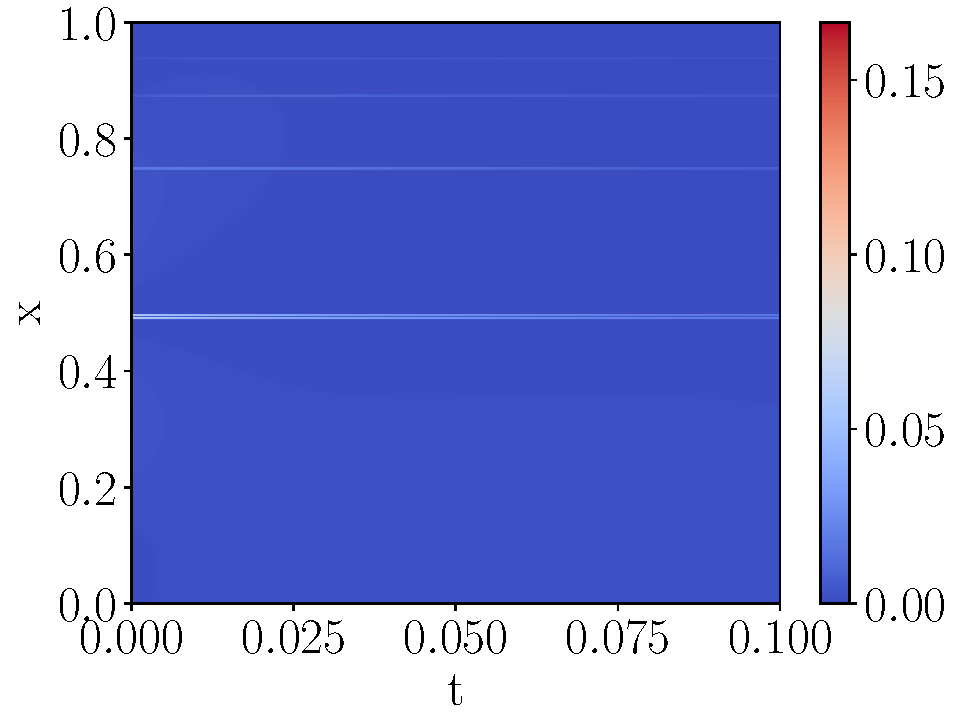
\includegraphics[width=\linewidth]{diff2d.pdf}
    \end{subfigure}
    \hspace{0.5cm}
    \begin{subfigure}{0.45\textwidth}
        \centering
        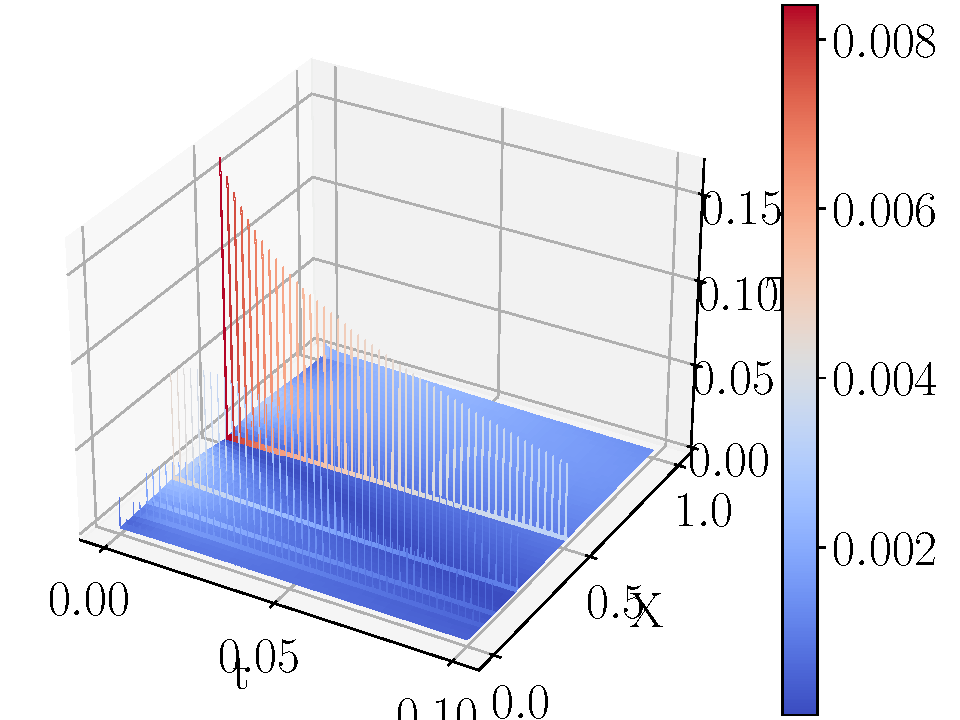
\includegraphics[width=\linewidth]{diff3d.pdf}
    \end{subfigure}
	\caption{Primerjava rešitev z Dirichletovimi robnimi pogoji s Fourirjevo metodo in metodo končnih diferenc pri 1000 položajnih korakih}
\end{figure}
Rezultati so precej nenavadni. Največja odstopanja se pojavijo na isti $x$ koordinati skozi čas, kar tvori nekakšne črte. V tri dimenzionalni predstavi pa opazimo, da imajo tako obliko le ena točka na celotnem območju, ki se zaradi načina vizualizacije na dvo dimenzionalnem grafu razširi. Relativno hitro lahko opazimo, da te napake izhajajo iz izračuna z metodo končnih diferenc, teh grafov tu ne prikazujemo, saj so enaki tistim iz Fourirjeve metode, napake pa brez interaktivnosti težko opazne. Omenimo tudi še zanimivo odvisnost, da če povečamo število korakov se tudi število črt odstopanj poveča.
\begin{figure}[H]
    \centering
    \begin{subfigure}{0.45\textwidth}
        \centering
        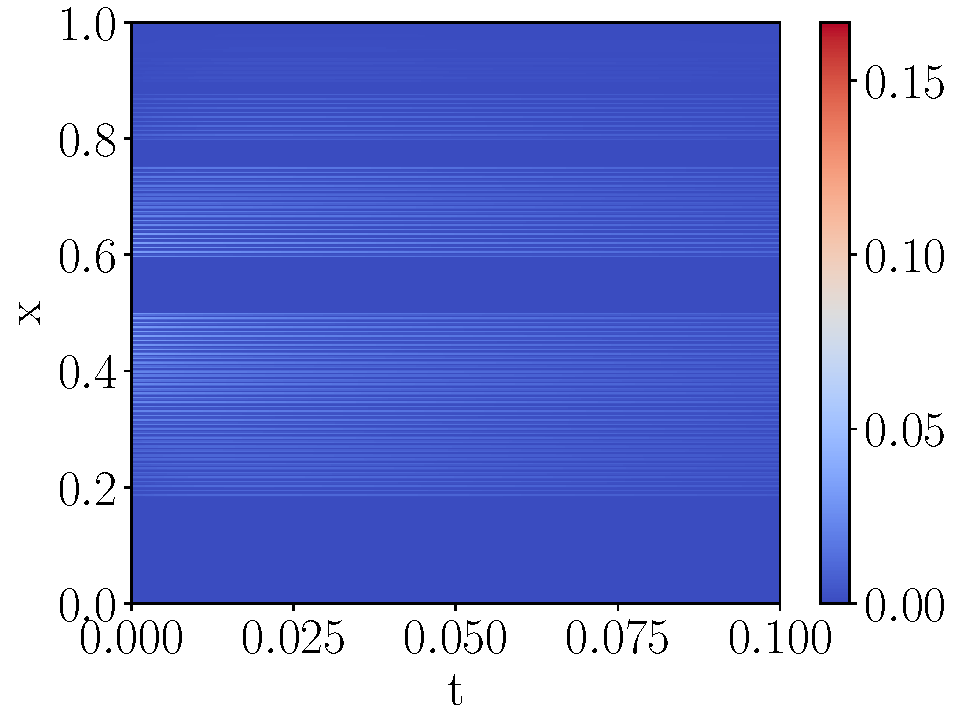
\includegraphics[width=\linewidth]{diffbigstep2d.pdf}
    \end{subfigure}
    \hspace{0.5cm}
    \begin{subfigure}{0.45\textwidth}
        \centering
        \includegraphics[width=\linewidth]{diffbigstep3d.pdf}
    \end{subfigure}
	\caption{Absolutna razlika rešitev z Dirichletovimi robnimi pogoji s Fourirjevo metodo in metodo končnih diferenc pri 10000 položajnih korakih}
\end{figure}
Ta anomalija pa sicer ni tisto kar nas najbolj zanima, a je edina vidna stvar na dobljenih grafih. Velika odstopanja teh točk namreč zakrijejo odvisnosti preostalega večinskega območja. Zato izključimo problematične točke in grafa poglejmo še enkrat.

\begin{figure}[H]
    \centering
    \begin{subfigure}{0.45\textwidth}
        \centering
        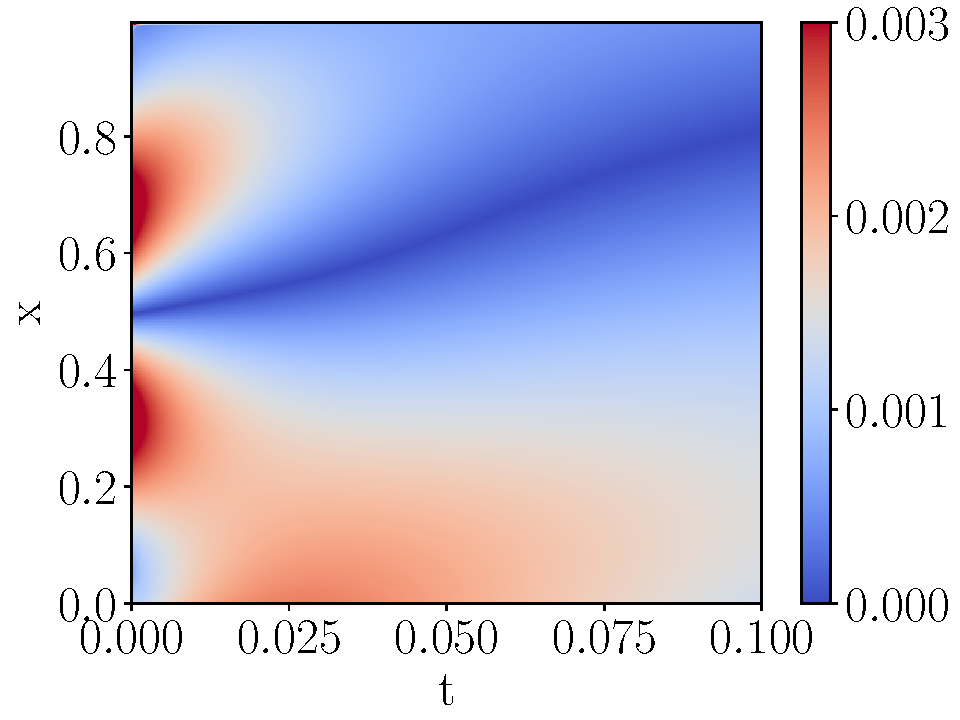
\includegraphics[width=\linewidth]{diffclean2d.pdf}
    \end{subfigure}
    \hspace{0.5cm}
    \begin{subfigure}{0.45\textwidth}
        \centering
        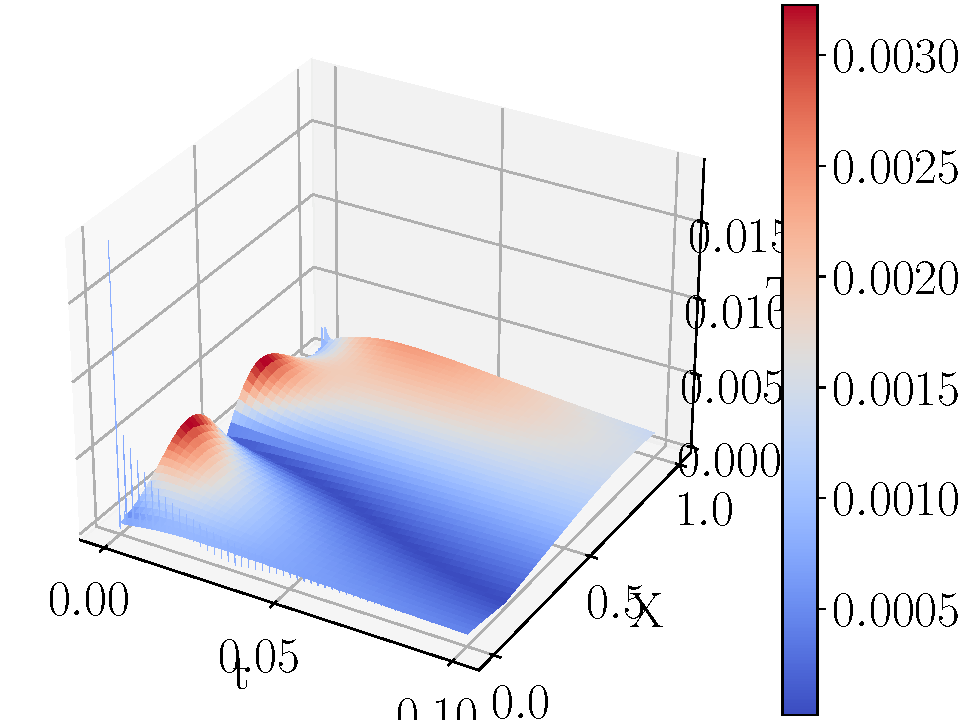
\includegraphics[width=\linewidth]{diffclean3d.pdf}
    \end{subfigure}
	\caption{Absolutna razlika z izključenimi problematičnimi točkami rešitev z Dirichletovimi robnimi pogoji s Fourirjevo metodo in metodo končnih diferenc pri 1000 položajnih korakih}
\end{figure}
Nov rezultat je nekako še bolj presenetljiv kot prejšnji. Intuitivno bi namreč pričakovali, da bodo odstopanja simetrična. Prva misel je, da morda z umikom nekaterih x koordinat podremo simetrijo. To hitro uvržemo, saj je asimetričnost prevelika glede na umaknjeno število točk in bi se ta tudi popravila pri risanju. Ko pomislimo kje v našem postopku uvedemo kakšno asimetrijo, je odgovor na to liha razširitev. Da bi to potrdili smo poskusili liho razširitev še nadaljevati tudi v drugo smer tako, da je naš začetni pogoj ponovno simetričen čez območje interesa. Nastali graf je precej podoben edina razlika je bila, da je bila asimetričnost nizkih vrednosti še precej bolj izrazita. To nakazuje, da je naše razmišljanje v pravi smeri, a je delovanje bolj zakomplicirano. 
\section{Zaključek}
Naloga je del serije reševanja parcialnih diferencialnih enačb. Zdela se mi je ena boljših nalog do sedaj, saj je spodbudila nekaj več razmišljanja o samem delovanju (hitre/diskretne) Fourirjeve transformacije. Poleg tega sem se tudi spoznal z B-zlepki. Dobil sem sicer rahlo nenavadne rezultate, kar namiguje, da se še kje skriva kakšna napaka in bi rabil porabiti še nekaj ur. A mislim, da so v splošnem odstopanja dovolj majhna, da se lahko zadovoljim z rezultatom.

\smallskip

Zapustil pa bi vas na novoletno-matematični noti z Nichomachusovim izrekom, ki trdi $\sum_{i=1}^{n} i^3 = \left(\sum_{i=1}^{n} i\right)^2$. Za $n=9$ pa se vrednost te enakosti izvrednoti ravno v naše novo leto $2025$. Več o tej enakosti pa si lahko \href{https://www.youtube.com/watch?v=ZWLkIW4NsQ0}{ogledate v tem videu}.
\end{document}
